\RequirePackage[T1]{fontenc}
\documentclass[conference,10pt,letterpaper]{IEEEtran}
\usepackage{amsmath,amssymb,graphicx,booktabs,cite}
\usepackage{algorithm,algpseudocode,tikz}
\usetikzlibrary{arrows.meta,positioning}
\usepackage{pgfplots}
\usepgfplotslibrary{groupplots}
\pgfplotsset{compat=1.18}
\usepackage[hidelinks]{hyperref}
\hypersetup{pdfauthor={},pdftitle={Exposing Inter-Sample and Intra-Search Parallelism in Layer-Aware Lookahead Construction for 3D FPGA Routing}}
\makeatletter
\newcommand{\tableinput}[1]{\@@input #1 }
\makeatother
\newtheorem{proposition}{Proposition}
\newcommand{\LstmPipeBuild}{$3.207\pm0.147\times$}
\newcommand{\LstmPipeProc}{$1.094\pm0.010\times$}
\newcommand{\LstmFlatBuild}{$3.208\pm0.165\times$}
\newcommand{\LstmFlatProc}{$1.092\pm0.007\times$}
\newcommand{\LstmAltCpuBuild}{$3.167\pm0.071\times$}
\newcommand{\LstmAltCpuProc}{$1.088\pm0.000122\times$}
\newcommand{\LstmStockBuild}{$21.182\pm1.342\times$}
\newcommand{\LstmStockProc}{$1.839\pm0.049\times$}
\newcommand{\StageProcBound}{1.005435}

\newcommand{\GemmNewPipeProc}{$1.102\pm0.004\times$}
\newcommand{\GemmNewStockProc}{$1.921\pm0.003\times$}
\newcommand{\GemmNewPipeBuild}{$3.643\pm0.091\times$}
\newcommand{\GemmNewStockBuild}{$23.524\pm0.120\times$}
\newcommand{\BnnNewPipeProc}{$1.098\pm0.009\times$}
\newcommand{\BnnNewStockProc}{$1.957\pm0.018\times$}
\newcommand{\BnnNewPipeBuild}{$3.197\pm0.116\times$}
\newcommand{\BnnNewStockBuild}{$20.619\pm0.248\times$}

\title{Exposing Inter-Sample and Intra-Search Parallelism in Layer-Aware Lookahead Construction for 3D FPGA Routing}
\author{\IEEEauthorblockN{Anonymous Authors}}
\begin{document}\maketitle
\begin{abstract}Layer-aware lookahead construction for 3D FPGA routing preserves source-relative delay and congestion costs, but its execution order can restrict parallelism both across samples and within a search. We expose these two granularities through context-preserving sample decoupling and whole-pair FP32 bucket waves. Private sample state and original-order reduction provide conditional native wire-map equivalence for STRICT CPU execution. ALT CPU/CUDA use a distinct wave selection rule, qualified separately through complete outputs and native routing. Matched scheduling controls identify cross-group parallelism, while wave profiles quantify concurrency versus repeated work. On new matched GEMM/BNN runs, CUDA achieves \GemmNewPipeProc\ and \BnnNewPipeProc\ complete-process speedups over eight-core Pipeline. A separate five-arm LSTM cohort gives $3.207\times$ construction and $1.094\times$ process speedups against Pipeline. Small-input slowdowns, representative-cost differences and cache applicability delimit these benefits.
\end{abstract}
\begin{IEEEkeywords}3D FPGA, routing lookahead, parallel algorithms, CPU/GPU, source-relative costs\end{IEEEkeywords}
\section{Introduction}
Three-dimensional and multi-die FPGAs expand the design space of programmable interconnects, while placing new demands on the CAD tools used to evaluate them. Recent frameworks support architecture generation, 3D placement and multi-die routing~\cite{lazagna,flatland,multidie}. Lookahead tables summarize delay/congestion costs by resource and destination context. Construction matters when architecture or cost changes invalidate an existing table. Compatible precomputed tables should be reused; our focus is the construction work that remains when such reuse is unavailable.

However, parallel routing does not automatically make lookahead construction parallel. In our locked VPR flow, a prior eight-core GEMM experiment spends 149.56 seconds constructing lookahead---approximately 45\% of its fixed-input process time. Two execution bottlenecks restrict concurrency: barriers between groups containing only a few samples, and fine-grained priority ordering within each search. Simply merging searches or relaxing their ordering is not a drop-in solution. Source/layer-relative recording context and associated delay/congestion representatives must survive reordering. The challenge is to separate removable scheduling constraints from output-defining dependencies.

MultiQueue-based routing parallelizes connection searches through carefully controlled priority relaxation~\cite{multiqueue}; it does not directly provide the sample-recording and reduction semantics of lookahead construction. Multi-die-aware lookahead improves how heuristic costs represent die crossings~\cite{multidie}, addressing the heuristic itself rather than the execution organization studied here. Parallel shortest-path methods already exploit buckets and frontier expansion to balance useful work against scheduling overhead~\cite{delta,gpu_sssp}. Lookahead additionally requires source-relative cells, coupled labels, same-bucket completion and native integration. Caching and sparse sampling can avoid or reduce construction~\cite{vproptions}; we parallelize the retained searches.

Our insight separates logical sample identity from execution order. STRICT schedules private samples across groups and reduces in native order under explicit equivalence conditions. ALT separately defines FP32 whole-pair waves within searches. Both integrate through logical sample/context boundaries, with CPU scheduling across samples and GPU waves within samples. The measured benefits extend beyond isolated kernels: STRICT Pipeline achieves a $1.638\times$ Process speedup over Stock on the prior eight-core GEMM cohort, while ALT CUDA achieves $3.207\times$ native construction and $1.094\times$ Process speedups over optimized CPU Pipeline on the same-family LSTM tuning holdout. These results are from separate cohorts. Our contributions are (C1) source-context-preserving cross-group decoupling with explicit reduction conditions, (C2) whole-pair FP32 wave execution with explicit closure and numeric limits, and (C3) native CPU/GPU integration with mechanism controls, route quality validation and measured applicability limits.

\section{Problem and Parallelism Boundary}
\subsection{Layer-Aware Construction}
Let $G=(V,E)$ be the directed routing-resource graph (RRG), with $N=|V|$ nodes and $M=|E|$ edges. Nodes carry resource type, layer, geometry and an indexed delay/congestion cost $w(v)=(d_v,q_v)$. The graph contains planar and cross-layer channels as well as logic, memory and DSP connectivity~\cite{third_dimension,multidie}. PathFinder-style negotiation resolves contention~\cite{pathfinder}; VPR consumes lookahead costs during routing~\cite{vtr8,vtr9}. We accelerate construction of the sampled wire table~\cite{diversity}, not negotiated routing itself.

A group $g=(\ell_s,\sigma,\tau)$ fixes source layer, segment type and channel type. Its ordered samples are source RR nodes $s_{g,j}$ with their native recording contexts. Flattening the native group/sample enumeration gives $J$ jobs indexed by $a$. A job retains its group $g(a)$, ordinal and source $s_a$. Each search can reach all target layers; the target layer is not a separate search. Its recording function $\phi_a(v)$ maps an eligible IPIN to the source-relative cell $u=(\ell_t,\Delta x,\Delta y)$, or to $\bot$ when native geometric filtering excludes it. For a grid of width $X$, height $Y$ and $L$ layers, the dense result domain contains $C=LXY$ cells per sample.

The per-sample result $R_a[u]$ is an occupied pair $(d,q)$ or a missing entry. Delay and congestion are associated representatives produced together by a search; they are not two independently optimized coordinates. Native strict-delay insertion $\oplus$ replaces a missing cell, or replaces an occupied pair only when the incoming delay is smaller. Thus, for each group,
\begin{equation}
 A_g[u]=\mathop{\bigoplus}_{a:g(a)=g}^{\text{native order}}R_a[u],\qquad
 F=\mathcal I\bigl(\mathcal C(\{A_g\})\bigr).
\end{equation}
Here $\mathcal C$ denotes the ordered native group writes and $\mathcal I$ their prescribed interpolation schedule, including missing-cell scan order. This notation represents the actual interleaving of writes and fills, not permission to commute them. The resulting table is indexed by $(\ell_s,\ell_t,\tau,\sigma,\Delta x,\Delta y)$. Source/OPIN preprocessing and derived minima remain in the native outer computation.

\subsection{Necessary Dependencies and Removable Barriers}
Source identity, eligibility, associated pairs and order-sensitive ties define the output. For starts at $x=0$ and $x=5$ reaching an IPIN at $x=6$ with delays 1 and 2, the contributions occupy displacement cells 6 and 1. A multi-source search retaining only the cheaper label at that IPIN loses the second contribution. Separately, inserting $(1,3)$ then $(1,9)$ must retain $(1,3)$ under native strict-delay reduction. Selecting delay and congestion independently could invent a pair no path produced.

In contrast, a search reads the shared graph/costs and its own source context, not another sample's mutable labels. Requiring all searches in group $g$ to finish before exposing group $g+1$ is therefore an execution barrier. Fine-grained priority extraction within a search is another constraint, but changing it also changes representative selection; it requires a separate semantic contract.

\subsection{Relation to Prior Parallelism}
MultiQueue routing controls priority relaxation in connection searches~\cite{multiqueue}; multi-die lookahead improves heuristic treatment of die crossings~\cite{multidie}. Neither directly supplies the sample-recording and ordered reduction boundary above. Delta-stepping and GPU SSSP establish bucket/frontier execution as a way to trade ordering overhead for parallel work~\cite{delta,gpu_sssp}. Our specialization retains source-relative cells, coupled cost representatives, closure and native consumption. oneTBB supplies execution primitives~\cite{tbb}; C1 concerns which dependencies those primitives may safely remove. Compatible caches and sparse-sampling \texttt{compressed\_map}~\cite{vproptions} address avoided work; our methods execute the retained samples. Section~\ref{sec:applicability} states their applicability boundaries.

\section{Two Levels of Dependency Decoupling}
\begin{figure}[t]\centering
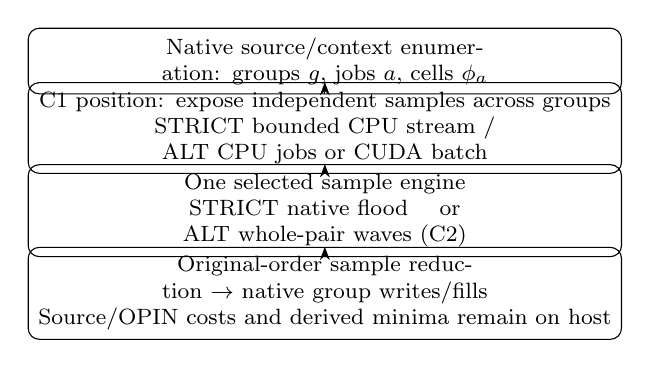
\begin{tikzpicture}[>=Stealth,every node/.style={draw,rounded corners,align=center,font=\footnotesize}]
\node[text width=7.3cm] (a) at (0,0) {Native source/context enumeration: groups $g$, jobs $a$, cells $\phi_a$};
\node[text width=7.3cm] (b) at (0,-0.85) {C1 position: expose independent samples across groups\\STRICT bounded CPU stream / ALT CPU jobs or CUDA batch};
\node[text width=7.3cm] (c) at (0,-1.9) {One selected sample engine\\STRICT native flood \quad or \quad ALT whole-pair waves (C2)};
\node[text width=7.3cm] (d) at (0,-2.95) {Original-order sample reduction $\to$ native group writes/fills\\Source/OPIN costs and derived minima remain on host};
\draw[->](a)--(b);\draw[->](b)--(c);\draw[->](c)--(d);
\end{tikzpicture}
\caption{Two parallelism levels within a common logical task boundary. Each configuration executes one search engine per sample; STRICT results are not fed into a second CUDA solve.}\label{fig:contracts}
\end{figure}

\subsection{C1: Private Samples and Ordered Consumption}
C1 separates source-context identity from execution order (Fig.~\ref{fig:contracts}). The STRICT Pipeline enumerates jobs in native order, exposes a bounded stream across all groups, and uses reusable worker-private queues, visited costs and expanded bits. Each sample resets its workspace and executes the native flood with unchanged geometry, edge eligibility and arithmetic. Its result is retained until the ordered consumer can merge it. The graph and indexed costs are shared read-only. No worker mutates another sample's labels or the group accumulator.

\begin{algorithm}[t]
\caption{C1: bounded STRICT sample execution}\label{alg:c1}
\begin{algorithmic}[1]
\State Enumerate groups and native sample starts into $\mathcal J$
\State Preserve each job's source, group and ordinal
\State Initialize group maps $A_g$; set token limit $K=\min(J,2P)$
\State Create thread-local reusable native search workspaces
\Statex \textit{Run these three stages as one bounded pipeline:}
\State \textbf{Ordered producer:} issue next job $a$ while a token is free
\State \textbf{Parallel worker:} reset private workspace $S_p$
\State \hspace{1em}$R_a\gets\mathrm{NativeFlood}(G,s_a,\phi_a,S_p)$
\State \hspace{1em}retain $(a,R_a)$ until its ordered consumption
\State \textbf{Ordered consumer:} for every cell $u$, perform
\State \hspace{1em}$A_{g(a)}[u]\gets A_{g(a)}[u]\oplus R_a[u]$
\State \hspace{1em}release sample result and its token
\State After join, write groups and interpolate in native order
\State Return wire table to remaining native outer computation
\end{algorithmic}
\end{algorithm}

The token bound follows the active CPU parallelism limit $P$ (at least one token when jobs exist). Searches from later groups can overlap earlier ones, while serial-in-order consumption preserves tie decisions. Flat is an independent global parallel-loop control: it retains all $J$ sample maps until the join and then reduces in original order. Group instead joins within every group. These are construction schedulers, not VPR's separate flat-routing option.

\begin{proposition}
If sample selection/context, within-flood visitation and arithmetic are unchanged, occupied recorded delays are finite, and native occupancy, commit and interpolation rules are preserved, private STRICT sample execution followed by original-order strict-delay reduction yields the native wire table.
\end{proposition}
\noindent\emph{Proof.} Each private flood produces the same per-cell representative as its native execution. For an occupied cell, ordered reduction selects the least delay and retains its earliest sample on equal delay:
\begin{equation}
 a^*(g,u)=\arg\min_{a:g(a)=g,\ R_a[u]\ne\bot}(R_a[u].d,a).
\end{equation}
The implementation uses the native missing-state predicate and insertion, not a generic tuple sort. Occupancy and associated congestion therefore agree cell by cell. Identical group writes and interpolation preserve this agreement. Completion order never enters the reduction. $\square$

Changing heap ties, exceptional-value handling or recording geometry violates the premises. The proposition is about wire maps, not route trajectories. ALT below changes the sample engine and does not inherit this proof.

\subsection{C1 Work, Width and Storage}
Let $t_a$ include sample reset, traversal and recording, and $W_g=\sum_{a:g(a)=g}t_a$. Ignoring launch, merge and interference, ideal search schedules obey
\begin{align}
 T_{\rm group}&\geq\sum_g\max\{W_g/P,\max_{a:g(a)=g}t_a\},\\
 T_{\rm global}&\geq\max\{\textstyle\sum_a t_a/P,\max_a t_a\}.
\end{align}
These are lower bounds, not speedup guarantees: an early slow sample can delay ordered consumption and occupy tokens. If $S(N)$ is native private workspace size including its queue, storage beyond the shared graph is $O(P S(N)+KC+|\mathcal G|C+J)$ for Pipeline; Flat replaces $KC$ by $JC$. This exposes the resource tradeoff of retaining independent results. Dense sample-to-group reduction performs $O(JC)$ cell visits; enumeration, group writes and interpolation add their own work. We do not assume a universal $O(M\log N)$ flood cost: actual queue traffic, termination and reset work depend on the native engine and graph.

\subsection{C2: Whole-Pair FP32 Waves}
ALT\_BUCKET\_FP32\_V1 makes the inner ordering rule explicit. A node label $L[v]=(d,q)$ is compared lexicographically:
\begin{equation}
 a\prec b\ \Longleftrightarrow\ a_d<b_d\ \lor\ (a_d=b_d\land a_q<b_q).
\end{equation}
Both coordinates of a winning proposal come from the same predecessor label plus the destination's indexed cost. This preserves pair association, but differs from native strict-delay ties. Initially $L[s_a]=(0,0)$ and other labels use an internal infinity sentinel. Output cells begin missing. The target count is the number of distinct mapped IPIN cells for that sample, not the number of target nodes.

The scheduling key is $B(d)=\mathrm{bits}_{32}(d)\gg h$. Native timings use $h=20$; $h=0$ is a diagnostic exact-delay-key control. Coarsening this key changes which labels are processed together, without quantizing their stored FP32 delays. Costs and generated candidates must be positive normal FP32 or positive zero: negative values, negative zero, subnormals, NaNs and infinities are rejected as numeric inputs/results. Infinity is only internal unreached state. CPU uses round-to-nearest with contraction/fast-math disabled; CUDA explicitly uses round-to-nearest addition. The admission pass checks inter-cluster non-SINK node costs and expansion checks each accumulated pair.

\begin{algorithm}[t]
\caption{C2: one logical ALT sample (native wave rule)}\label{alg:c2}
\begin{algorithmic}[1]
\State Reset labels, pending keys, closed-set flags and cell output
\State Count distinct target cells; if zero, return missing output
\State Publish $s_a$ with label $(0,0)$ and key 0
\While{pending work exists}
\State $b\gets$ minimum pending key; extract its members
\State Discard stale members whose current pending key is not $b$
\State Clear valid members' pending keys; add them to closed set
\State Freeze committed labels $L$ for this wave
\State Initialize touched-node proposals $Q[v]\gets L[v]$
\For{each active $u$ and its adjacency in stored order}
\State Apply native eligibility; skip or stop at SINK as specified
\State $z\gets\mathrm{RN}_{32}(L[u]+w(v))$; reject invalid numerics
\State $Q[v]\gets\min_{\prec}(Q[v],z)$ as a whole pair
\EndFor
\State After expansion, commit every strict $Q[v]\prec L[v]$
\State Publish its new key, deduplicating current notifications
\If{minimum remaining key differs from $b$, or none remains}
\State Reduce closed IPIN labels into their mapped output cells
\State Clear closed set; stop if all target cells are recorded
\EndIf
\State Fail explicitly if the execution/capacity guard is exceeded
\EndWhile
\State Return output with missing unreachable cells; no partial success on error
\end{algorithmic}
\end{algorithm}

A coarse bucket can contain a later improvement to a node already expanded. Therefore processing it once and permanently marking it visited is wrong for this execution rule. Clearing the active pending key permits re-publication into the same bucket. CPU keeps historical directory entries, rejects stale keys and suppresses duplicate current keys. CUDA stores one current pending key per node, replacing a migrated key directly. A bucket closes only after no current pending key remains at $b$; the closed set accumulates expanded nodes until that boundary. IPIN output reduction then selects whole pairs and tests target completion. Queue exhaustion also terminates with unreachable cells missing.

Expansion reads wave-start labels and writes a distinct proposal array; commit follows all expansion. Without that boundary, a newly written label could propagate further within the same wave depending on thread timing. In CUDA, proposals persist as running minima rather than being reset each wave: after commit they equal the committed labels, which provides the same starting value for the next expansion. This is the measured dense implementation, not a later online reduction variant. Pair preservation is not a universal lexicographic FP32 shortest-path theorem: rounding can collapse previously different delays, altering which congestion tie would have survived.

\subsection{CPU/GPU Mapping and Costs}
ALT CPU receives the full job list through the live native interface. An OpenMP dynamic loop assigns independent samples to private scratch arrays with a sparse ordered map of pending buckets. It does not call the STRICT TBB Pipeline. CUDA allocates all $J$ samples together: grid dimension $y$ identifies the sample, while $x$ and 256-thread blocks identify nodes. Each active node thread loops over its own adjacency. Candidate edges are not each assigned a separate thread.

For admitted nonnegative floats the unsigned key
\begin{equation}
 H(d,q)=(\mathrm{uint64}(\mathrm{bits}_{32}(d))\ll32)
          \mathbin{|}\mathrm{bits}_{32}(q)
\end{equation}
orders complete pairs. CUDA uses a 64-bit atomic minimum on each destination proposal; collisions select one actual candidate pair. Separate expansion, commit/minimum-scan, confirmation and advance kernels provide wave boundaries. The commit scan reduces pending keys within each block before one atomic minimum per block; confirmation records IPIN pairs only at closure. Advance scans output occupancy per sample. A host completion-count copy waits each batch round, followed by device synchronization and full output readback/unpacking. The contexts field configures CPU workers; it does not measure CUDA occupancy.

Let $A_{a,k}$ be active nodes, $E_{a,k}$ actually inspected adjacency entries (including rejected edges), $U_{a,k}$ touched destinations and $D_{a,k}$ directory operations in wave $k$. CPU work includes initialization $O(J(N+C))$, $\sum_{a,k}(|A_{a,k}|+|E_{a,k}|+|U_{a,k}|)$, stale-entry filtering, closed-set recording and ordered-directory costs $O(\sum_{a,k}D_{a,k}\log(1+B_{a,k}))$, where $B_{a,k}$ is the number of live directory buckets. Repeated waves can inspect an edge many times. GPU work additionally includes dense scans over allocated $JN$ slots each batch round and closure output scans; for $W$ rounds a useful accounting is
\begin{equation}
 O\!\left(J(N+C)+WJN+\sum_{a,k}|E_{a,k}|+\sum_a H_a C\right),
\end{equation}
where $H_a$ counts closure occupancy scans. Atomic contention, launches and host waits affect elapsed time beyond this work count. Neither formula assumes a single visit per edge.

For the original CUDA representation, arrays require $25JN+8JC$ bytes for labels/proposals, pending, closed flags, mapping and output, plus $8(N+1)+16N+8M$ for CSR/nodes/edges and cost/job metadata. Admission estimates the complete allocation and requires it to fit within 80\% of free device memory; allocation/API errors remain failures. Native ABI shape checks and finite wave/time guards further bound execution. Earlier ALT qualification used $N<2^{23}$; the unchanged live ALT ABI admits the new 9,595,752-node GEMM input, which separately passes full CPU/CUDA and native-route qualification. The tighter historical envelope is not an enforced live ALT node limit. No sample reduction or automatic batching is part of these results.

The host exports current graph/costs and per-sample geometry, calls exactly one chosen backend, then merges returned samples in original order and completes native writes/interpolation. Graph conversion, allocation, transfer, synchronization and output handoff are charged to native E2. Table~\ref{tab:configs} distinguishes executable choices from the two mechanisms. Stock$\to$Pipeline$\to$ALT CUDA is an implementation comparison; it is not a serial two-solver flow or a complete $2\times2$ causal ablation.

\begin{table}[t]\centering
\caption{Execution choices at the common logical boundary.}\label{tab:configs}
\begin{tabular}{lp{2.35cm}p{3.60cm}}\toprule
Configuration & Across samples & Within sample / guarantee\\\midrule
STRICT CPU & Group, Flat or bounded Pipeline & Native flood; conditional wire-map equality\\
ALT CPU & Global dynamic jobs & FP32 waves; separate numeric/QoR qualification\\
ALT CUDA & Full sample batch & Node threads and atomic pairs; ALT CPU output qualification\\\bottomrule
\end{tabular}\end{table}

\section{Experimental Method and Evidence}
\subsection{Frozen Inputs, Cohorts and Resources}
Construction-only controls use separately bound RRGs; capped route tails do not establish legality. Historical native BNN/s38417 compare Stock, Flat, ALT CPU and original ALT CUDA. LSTM seed2 adds Pipeline on another cohort. Previously used in the CPU study, LSTM is a same-family holdout from preceding ALT tuning, frozen before its own tests, not before all ALT development. It shares BNN's architecture but has a different netlist, placement and RRG.

New matched GEMM/BNN runs retain their original seed1 inputs: width100 for GEMM, width120 for BNN. LSTM also uses width120; all three have two layers and 40 samples (Table~\ref{tab:qor}). The new allocation fixes eight physical cores and NUMA0 memory binding on a Xeon Platinum 8462Y+, one H100 80GB, a 10-CPU quota and 200GiB RAM. The earlier native ALT cohorts use eight physical cores in one NUMA node on Gold 6530 and one H100 80GB. Solvers execute sequentially, with rotated arm order and fresh processes. Shared hosts are not exclusive; cohorts are not pooled. The baseline is VTR commit \texttt{0b912334fdd8}, release build, assertion level 2.

\subsection{Timing and Statistical Policy}
E1 is sample service; CUDA ends it before final ABI output copy. E2 is native \texttt{MapLookahead::compute}: conversion, preparation/service, output handoff, group merge, interpolation, source/OPIN and derived minima. Process adds RR XML loading, initialization, routing, checking/STA and uniform serialization. Independent route readback, pre-generated RRG, packing and placement are excluded. Caches are not flushed.

For paired repeat $r$, $s_r=T_{c,r}/T_{a,r}$. We report mean and sample SD of ratios and raw seconds ($n=3$). SD is not a confidence interval; repeats are processes, not designs or seeds. Stock E2 precision is 0.01s; other E2 timers are high resolution. Profiles are outside formal timing.

\subsection{Qualification and Attribution}
STRICT checks wire-map bytes under its proposition. ALT checks complete CPU/CUDA pairs and maps, then each route through independent original-VPR FULL/STA with unchanged route SHA, zero overuse, and CPD/wirelength within $+5\%$ of controls: Flat/Stock for LSTM, Stock/Pipeline for new GEMM/BNN. New ALT CPU runs are qualification-only; formal CUDA disables capture and CPU-reference verification.

Retained bounding-box notification repairs can change route trajectories despite identical maps; a unique complete cause is not established. Stock ratios describe the implementation combination. Shared-repair Flat/Pipeline/ALT comparisons better isolate construction.

\section{Results and System Interpretation}
\subsection{STRICT Cross-Sample Parallelism}
On the prior eight-core GEMM cohort, STRICT Pipeline reduces construction from 149.56 to 20.95 seconds and achieves $1.638\pm0.005\times$ paired Process speedup over Stock; Group takes 37.88 seconds. Construction is about 45\% of Stock Process. Matched Group/Flat/Pipeline controls isolate C1 from other Stock repairs.

\begin{figure}[t]\centering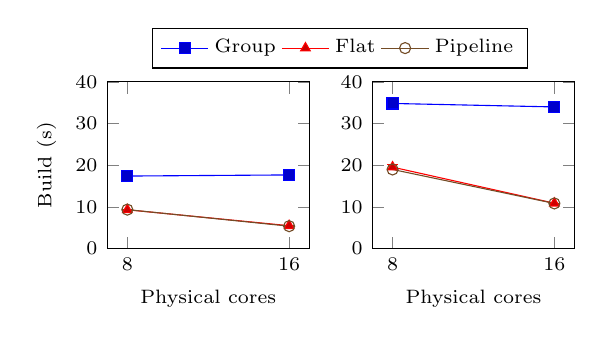
\begin{tikzpicture}
\begin{groupplot}[group style={group size=2 by 1,horizontal sep=0.8cm},width=4.15cm,height=3.7cm,xtick={8,16},xmin=7,xmax=17,ymin=0,ymax=40,xlabel={Physical cores},ylabel={Build (s)},label style={font=\scriptsize},tick label style={font=\scriptsize},legend style={font=\scriptsize,at={(1.15,1.08)},anchor=south,legend columns=3},error bars/y dir=both,error bars/y explicit]
\nextgroupplot[title={},ylabel={Build (s)}]
\addplot+[mark=square*] coordinates {(8,17.413333333333334) +- (0,0.3250128202599597) (16,17.683333333333334) +- (0,0.3257811126098835)};
\addplot+[mark=triangle*] coordinates {(8,9.32) +- (0,0.15394804318340596) (16,5.506666666666667) +- (0,0.030550504633038766)};
\addplot+[mark=o] coordinates {(8,9.363333333333333) +- (0,0.10598742063723142) (16,5.3933333333333335) +- (0,0.08082903768654771)};
\legend{Group,Flat,Pipeline}
\nextgroupplot[title={},ylabel={}]
\addplot+[mark=square*] coordinates {(8,34.82333333333333) +- (0,0.3181718613160717) (16,33.99) +- (0,0.6602272336097627)};
\addplot+[mark=triangle*] coordinates {(8,19.553333333333335) +- (0,0.6217180497084931) (16,10.896666666666667) +- (0,0.040414518843273746)};
\addplot+[mark=o] coordinates {(8,18.993333333333332) +- (0,0.11503622617824955) (16,10.846666666666668) +- (0,0.04041451884327389)};
\end{groupplot}
\end{tikzpicture}

\caption{Construction means and sample SD, three processes per arm/point. Same-cohort Group/Flat/Pipeline controls on BNN (left) and DLA (right); capped routing tails do not establish full-route legality. Error bars are small at this scale.}\label{fig:causal}\end{figure}

In Fig.~\ref{fig:causal}, ten groups of four samples limit group-local concurrency. At eight cores, BNN Group/Flat/Pipeline take $17.41\pm0.33$, $9.32\pm0.15$ and $9.36\pm0.11$ s. Flat and Pipeline independently remove barriers and are nearly equal: the benefit comes from decoupling groups, not a particular Pipeline primitive. At sixteen cores Flat/Pipeline take 5.51/5.39 s, against Group's 17.68 s. DLA shows the same mechanism (34.82/19.55/18.99 s at eight cores). Separate 2D controls also benefit: eight-core BNN-2D takes 7.75/4.23/4.16 s. These are not equal-sized 2D/3D pairs, so layer count is not a causal explanation of time differences.

\subsection{Wave Scheduling: Concurrency Versus Work}
\begin{table}[t]\centering\caption{Matched BNN40 original-representation profiles; diagnostic operation counts, not native E2 timing.}\label{tab:waves}
\begin{tabular}{lrr}\toprule Metric & Shift 0 & Shift 20\\\midrule
\tableinput{tables/waves.tex}\bottomrule\end{tabular}\end{table}
Table~\ref{tab:waves} recomputes complete per-sample profiles. Shift 20 reduces summed waves by $9.112\times$ and maximum per-sample waves (the corresponding batch rounds) by $10.627\times$, while increasing eligible edge work only $0.3504\%$. Edge-work-weighted frontier grows $6.6484\times$. This exposes more work per synchronization opportunity; it is neither an occupancy measurement nor proof that launches explain all runtime. Labels remain FP32 and shift-0/20 complete CPU/CUDA outputs agree under ALT. Instrumented profile times are excluded from native statistics. Semantic fixture checks include eight random cases with native congestion differences, motivating separate semantic/QoR qualification.

\subsection{Matched Native Process and Construction}
\begin{table*}[t]\centering\caption{Complete native Process seconds and directly paired speedups, mean $\pm$ sample SD ($n=3$). S: Stock; P: Pipeline; C: ALT CUDA. GEMM/BNN are one new allocation; LSTM is a separate historical cohort.}\label{tab:matchedproc}
\begin{tabular}{lrrrrrr}\toprule Workload & Stock (s) & Pipeline (s) & ALT CUDA (s) & S/P & P/C & S/C\\\midrule
\tableinput{tables/matched_process.tex}\bottomrule\end{tabular}\end{table*}
\begin{table*}[t]\centering\caption{Native lookahead construction E2 seconds and directly paired speedups for the same runs as Table~\ref{tab:matchedproc}; mean $\pm$ sample SD, $n=3$.}\label{tab:matchede2}
\begin{tabular}{lrrrrrr}\toprule Workload & Stock (s) & Pipeline (s) & ALT CUDA (s) & S/P & P/C & S/C\\\midrule
\tableinput{tables/matched_e2.tex}\bottomrule\end{tabular}\end{table*}
CUDA/Pipeline E2 ratios are \GemmNewPipeBuild\ for GEMM and \BnnNewPipeBuild\ for BNN (Tables~\ref{tab:matchedproc}--\ref{tab:matchede2}). Their Process ratios, \GemmNewPipeProc\ and \BnnNewPipeProc, are smaller because Process retains loading, initialization, routing and checking. Ratios use matched rounds, never historical denominators. These implementation comparisons are not a complete two-factor ablation.

\subsection{Native LSTM: Five Matched Configurations}
\begin{table}[t]\centering\caption{Historical LSTM native seconds, mean $\pm$ sample SD ($n=3$); five arms on its own rotated eight-core/H100 cohort.}\label{tab:lstm}
\begin{tabular}{lrr}\toprule Method & E2 & Process\\\midrule
\tableinput{tables/lstm.tex}\bottomrule\end{tabular}\end{table}
CUDA obtains \LstmPipeBuild\ E2 and \LstmPipeProc\ Process acceleration against Pipeline; against Flat, \LstmFlatBuild\ and \LstmFlatProc; against matched ALT CPU, \LstmAltCpuBuild\ and \LstmAltCpuProc. ALT CPU is close to Pipeline: changed search semantics alone do not explain GPU acceleration. 

\subsection{Semantics, QoR and Size Dependence}
\begin{table}[t]\centering\caption{Native qualification: nodes/edges in millions; CPD/WL changes (\%) against Stock; $\Delta q$ counts final-map congestion-word changes against STRICT. All cases have two layers and 40 samples; LSTM is historical.}\label{tab:qor}
\begin{tabular}{lrrrrr}\toprule Case & $N/10^6$ & $M/10^6$ & CPD & WL & $\Delta q$\\\midrule
\tableinput{tables/qualification_compact.tex}\bottomrule\end{tabular}\end{table}
Complete ALT CPU/CUDA samples and maps agree on each input. Stock/Pipeline maps also agree, while ALT changes congestion representatives: 50,789 GEMM, 24,434 BNN and 23,111 LSTM words, with zero delay or missing-state differences. Native strict-delay ties and ALT whole-pair improvement remain distinct contracts. Each route independently passes FULL/STA with unchanged own route SHA and zero overuse; equivalent maps do not require identical route SHAs. Every new formal run passes the $+5\%$ CPD/WL gate against both paired controls; this is not a universal zero-loss guarantee.

The separate historical BNN Flat/CUDA cohort gives $3.274\pm0.222\times$ E2 and $1.091\pm0.011\times$ Process ratios; it supplies no denominator for the new Pipeline comparison. Its s38417 negative case remains $0.274\pm0.032\times$ E2 and $0.912\pm0.016\times$ Process. Device initialization, scans and launches can outweigh a small build. ALT CPU improves construction there, but Stock is fastest for Process; no automatic size selector or all-size benefit is established.

\subsection{Closest Alternative and Cache Applicability}\label{sec:applicability}
The locked executable exposes \texttt{compressed\_map}, whose embedded assertion and compute source require one layer; the evaluated native graphs have two. This is a static domain exclusion, not a timed failure or superiority claim over supported configurations. Its compressed reader and binary writer are unimplemented (CSV export is separate). Separable is exposed but not qualified or timed here. For ordinary map caching, 36 historical fixed-input reuse records have legal routing and independent FULL/STA checks. They establish valid cache hits, separate from fresh construction; no unobserved cross-design reuse is amortized.

\subsection{Resident Time Has a Different Scope}
A separate packed resident cohort excludes host preparation/full readback. Dual Gold 6530 uses 64 cores with a 55-CPU quota; 40 samples cap concurrency at 40. Among 8/32/64 workers, 64 gives the lowest means: $0.699624\pm0.026647$ s for BNN40 and $0.725510\pm0.021287$ s for LSTM40 (three processes, each averaging three repetitions after one warmup). H100 resident means are 0.151800/0.159498 s, including initialization, launches/control and completion synchronization. The BNN GPU record lacks an execution-time executable digest. These different representations/resources/scopes do not strengthen native E2/Process speedups.

\section{Scope and Limitations}
STRICT equality remains conditional; ALT route qualification covers tested graphs, not a universal QoR bound. Three process repetitions, shared hosts and same-family architectures limit generalization. Controls and ALT retain RRG no-fanin diagnostics: FULL/STA validates actual routes, not every graph-generation choice. Dense state, scans and launch costs bound GPU applicability. Construction-only, eight-core native and packed resident results retain separate scopes. The evidence supports complementary mechanisms, not independent multiplicative C1/C2 effects or an automatic backend selector.

\section{Conclusion}
Source-context preservation separates private sample execution from ordered reduction, while FP32 whole-pair waves expose work within each search. Native integration charges conversion and outer construction. CUDA gives \GemmNewPipeProc\ and \BnnNewPipeProc\ Process ratios against eight-core Pipeline on matched GEMM/BNN; historical LSTM gives \LstmPipeProc. Mechanism controls and the small-input negative case delimit these gains. ALT remains separately qualified, without inheriting STRICT equivalence.

\section*{Content Generated by AI}
OpenAI Codex (GPT-6) assisted manuscript text, figures, artifact scripts and experimental analysis. Authors are responsible for verification and submission.

\clearpage
\bibliographystyle{IEEEtran}
\bibliography{references}
\end{document}
